\section{Preliminaries}
\label{sec:preliminaries}

\subsection{Background}
\label{sec:background}

An attributed graph $G = (V,E,L)$ has a set of nodes $V$, a set of edges
$E \subseteq V \times V$, and a label set $\mathbb{L}$ such that
every node $v \in V$ is associated with a label, i.e., $L(v) \in \mathbb{L}$.
In this work, we focus on bidirectional, node-labeled, and un-weighted
graphs. However, the proposed models and algorithms can also be applied to directed
and edge-labeled graphs.

\spara{Subgraph Isomorphism.} Given an input graph $G=(V,E,L)$, a graph pattern
$Q=(V_Q,E_Q,L_Q)$, a subgraph isomorphism is an {\em injective function} $M: V_Q \rightarrow V$ s. t.
(1) $\forall v\in V_Q, L_Q(v)= L(M(v))$, and (2) $\forall(v_1,v_2) \in E_Q, (M(v_1),M(v_2))\in E$.

Subgraph isomorphism is depicted in Figure~\ref{fig:subgraph_isomorphism}. $M$ is called a subgraph-isomorphic
{\em mapping}. The nodes $\{M(v):v\in V_Q\}$ and the corresponding edges $\{(M(v_1),M(v_2)):(v_1,v_2)\in E_Q\}$
form a subgraph-isomorphic {\em instance} of $Q$ in $G$.
There can be many subgraph-isomorphic mappings and instances of $Q$, e.g., in Figure~\ref{fig:subgraph_isomorphism}
another mapping $M_1$ could be as follows: $M_1(v_1)= u_3$, $M_1(v_2)= u_2$, $M_1(v_3)= u_7$. Clearly, two different
instances of the same pattern may overlap, as in our current scenario: the two instances, defined by mappings $M$
and $M_1$, overlap at nodes $u_2$ and $u_3$,
and also on the edge $(u_2,u_3)$.
%
\begin{figure}[t!]
\centering
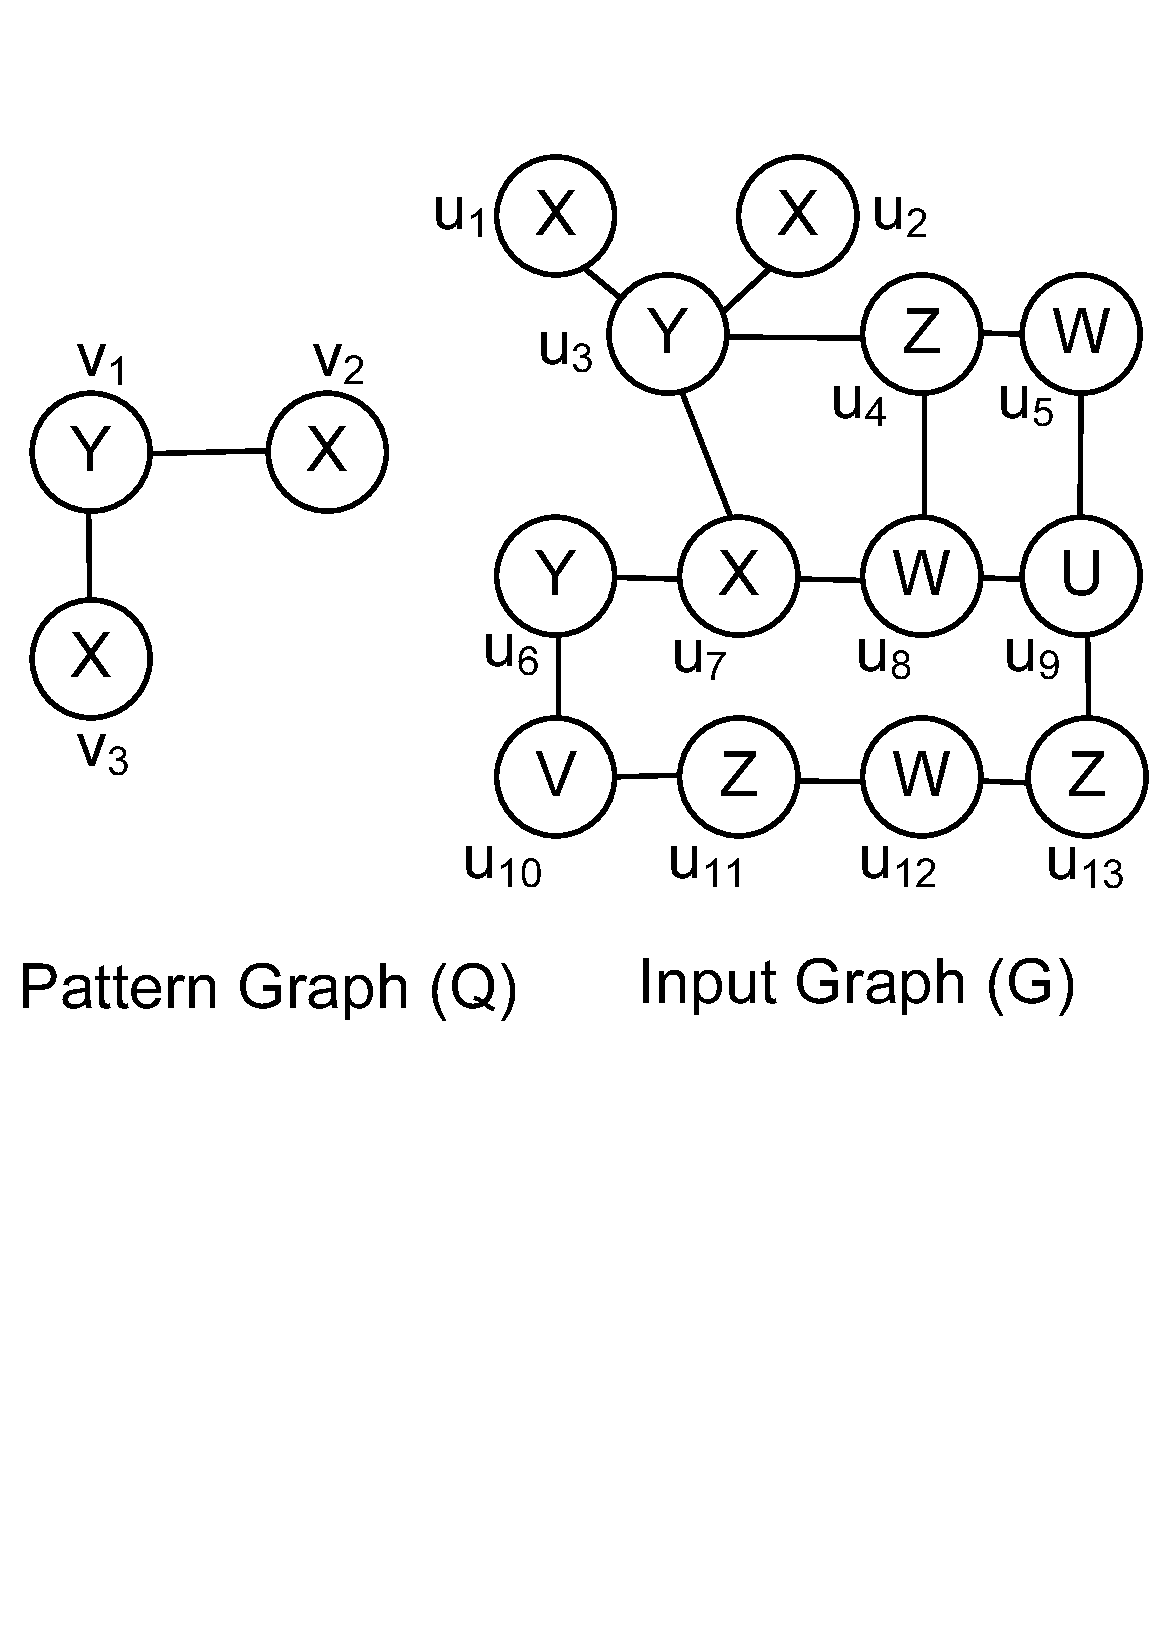
\includegraphics[scale=0.23]{images/subgraph_isomorphism}
\vspace{-2mm}
\caption{\small Subgraph isomorphism: $M(v_1)= u_3$, $M(v_2)= u_1$, $M(v_3)= u_2$. Two other subgraph-
isomorphic mappings could be as follows: $M_1(v_1)=u_3$, $M_1(v_2)=u_1, M_1(V_3)=u_7$; and
$M_2(v_1)=u_3, M_2(v_2)=u_2, M_2(v_3)=u_7$.}
\label{fig:subgraph_isomorphism}
\vspace{-5mm}
\end{figure}

\spara{Support.}
To find frequent subgraphs from a single, large graph, existing literature 
proposed several definitions of subgraph support, denoted as $\sigma$, e.g., maximum independent sets (MIS) \cite{KK04}, 
minimum image-based (MNI) \cite{BN08}, and harmful overlap (HO) \cite{FB07}.
All these metrics are {\em downward-closure}: The support of a supergraph 
$Q_1 \succeq Q$ is higher than that of its subgraph $Q$, i.e., $\sigma(Q_1) > \sigma(Q)$.
However, these metrics differ in the amount of overlap that they allow between subgraph-isomorphic 
instances, and in the complexity of their computation.

In this work, we adopt MNI  \cite{BN08}
due to the following reasons. First, the MNI support
can be efficiently computed; whereas the computation of MIS and HO are \NP-complete \cite{KK04,FB07}.
Second, MNI provides a superset of the results of the two other metrics; thus
the MIS or HO-based results can be identified via an expensive post-processing step,
which prunes out the unqualified subgraphs \cite{EASK14}.
Next, we formally define the MNI support.

\spara{Minimum Image-based (MNI) Support.} Bringmann and Nijssen \cite{BN08} developed the
minimum image-based support. It is based on the number of unique nodes in $G$ that a node of the pattern $Q$
is mapped to. Formally,
%
\begin{align}
\displaystyle \sigma(Q) = \min_{v \in V_Q} |\{M(v) : M \,\text{is a subgraph-isomorphic mapping}\}| &
\end{align}

In Figure~\ref{fig:subgraph_isomorphism}, the MNI support of $Q$ is $1$, which is due to
node $v_1$ having label $Y$, it is mapped to only one node in $G$, i.e., $u_3$ for all three
mappings. The nodes in the set $\{M(v)\}$ for different mappings $M$ are called the {\em images} of $v$.

\spara{Frequent Subgraphs.} Given the input graph $G$, a user-defined minimum-support threshold {\sf Min-Sup}, and
a definition of support $\sigma$, the frequent subgraphs mining problem identifies all subgraphs $Q$ of $G$, such that
$\sigma(Q)\ge$ {\sf Min-Sup}.

\subsection{Problem Formulation}
\label{sec:problem}

Informally speaking, our objective is to identify those pairs of subgraph patterns $\langle Q_1, Q_2\rangle$ such that
they occur closely for a sufficiently large number of times in the input graph $G$. We formalize this notion of
correlation by incorporating the following constraints: (1) The correlation between two subgraph patterns must be
symmetric, and (2) it shall be consistent with respect to the notion of MNI support. 

To be consistent with the MNI support, we group subgraph instances as follows.

\begin{defn}[Instance Grouping]
\label{def:instance_grouping}
Given the input graph $G$, a graph pattern $Q$, and its instances in $G$ denoted as $\mathbb{I}=\{I_1,I_2,\ldots,I_s\}$,
let us define by $v^*$ the node in $Q$ which has the minimum number of images. We denote by
$M(v^*)=\{M_1(v^*),M_2(v^*),\ldots,M_{\sigma(Q)}(v^*)\}$ the images of $v^*$. Notice that
$\sigma(Q)$ is the MNI support of $Q$, $\sigma(Q)\le s$, and $M_j$ is
a mapping of $Q$, for all $1 \le j \le \sigma(Q)$. Next, we form a grouping
of instances, denoted as $\mathbb{I'}=\{I'_1,I'_2,\ldots,I'_{\sigma(Q)}\}$, where
$I'_j= \{I:M_j(v^*) \in I, I \in \mathbb{I}\}$. Intuitively,
$I'_j$ is the group of instances containing the image node $M_j(v^*)$.
\end{defn}
%
\begin{exple}
For input graph $G$ and graph pattern $Q_1$ in Figure~\ref{fig:correlation},
the instances are
given by $\mathbb{I}=\{u_1u_3,u_2u_3,u_7u_3,u_7u_6\}$. However, its MNI support is two, since
node $v_2$ has only two corresponding images: $u_3$ and $u_6$. Thus, we group the instances
according to the presence of $u_3$ and $u_6$ as follows: $\mathbb{I'}=\{u_1u_2u_7u_3,u_7u_6\}$.
\end{exple}

\begin{figure}[t!]
\centering
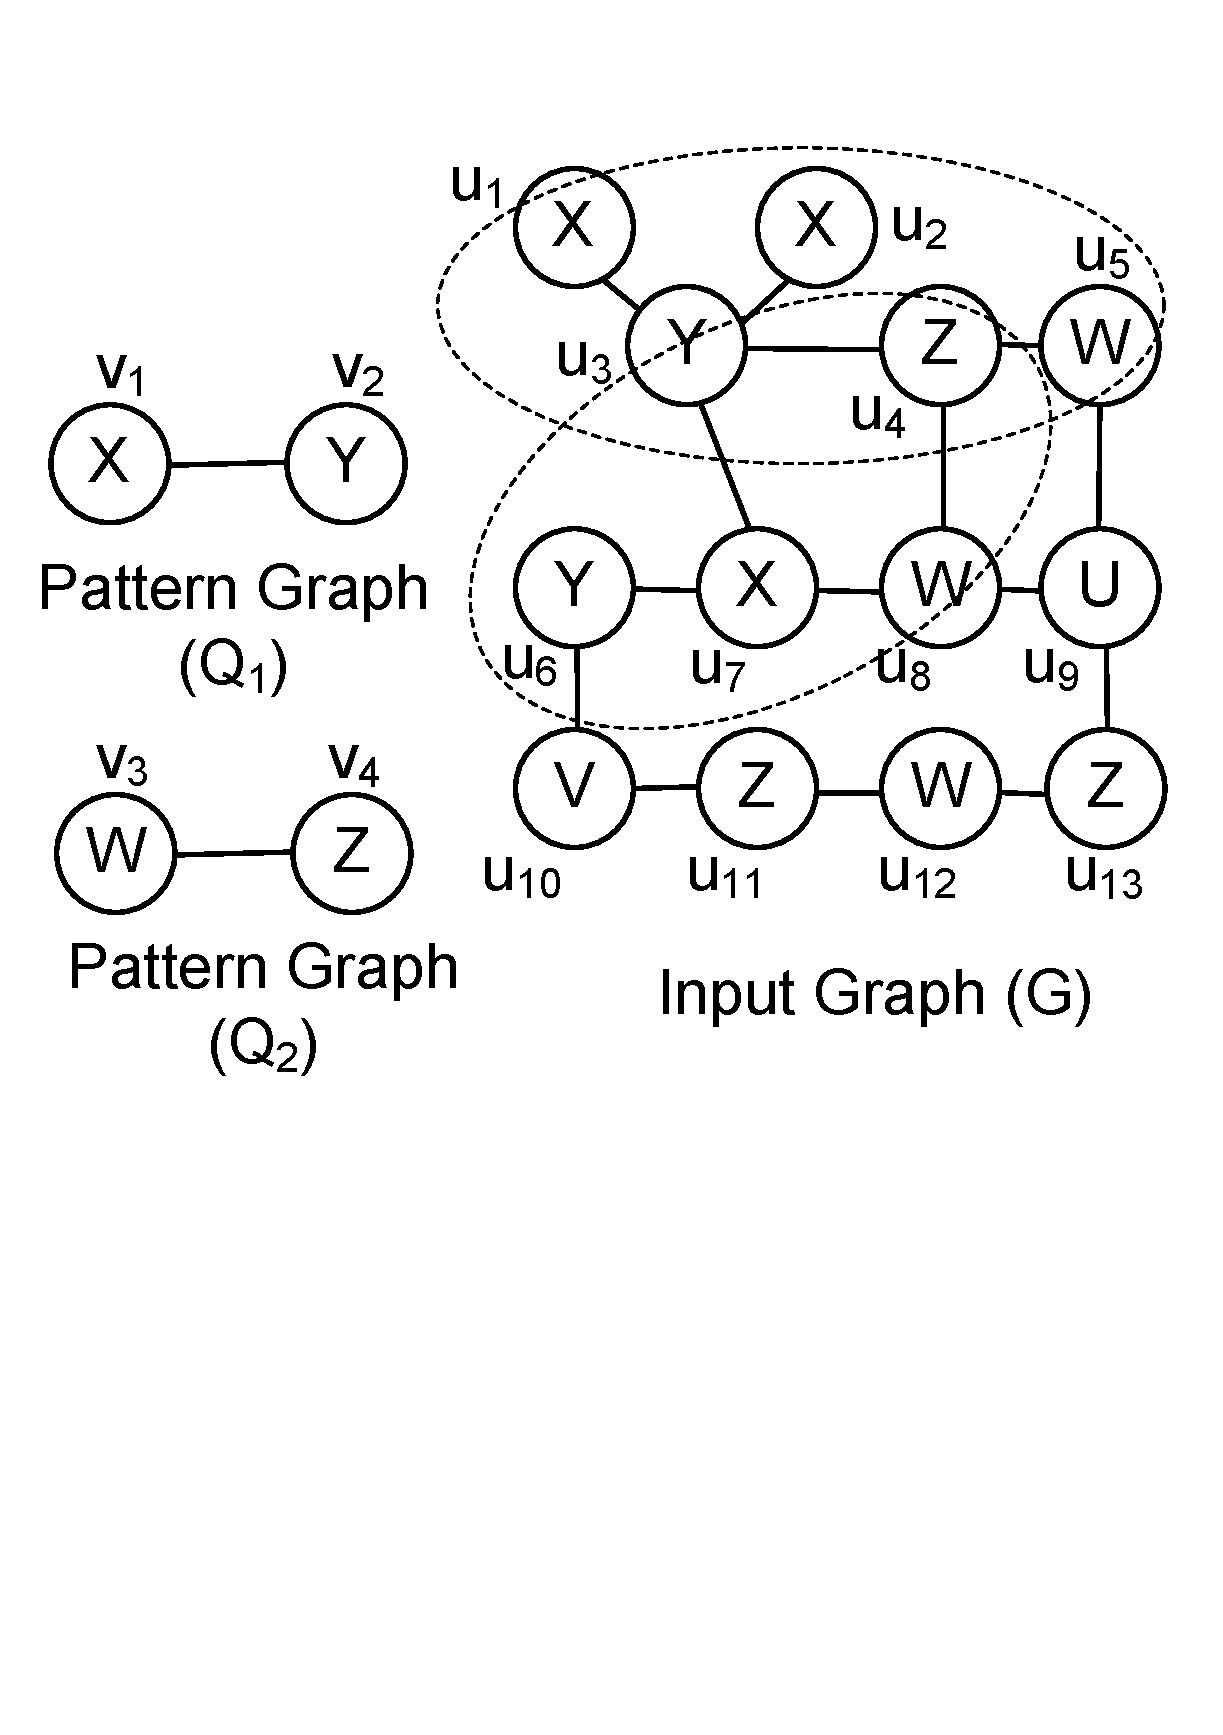
\includegraphics[scale=0.23]{images/correlation}
\vspace{-2mm}
\caption{\small Correlation between subgraphs $Q_1$ and $Q_2$ in $G$}
\label{fig:correlation}
\vspace{-5mm}
\end{figure}

Note that the grouping is not a partition of instances. It is possible for an instance 
to belong to multiple groups, especially when the pattern has multiple nodes with the same label. 
However, for a pattern $Q$, we ensure that the number of instance-groups would be $\sigma(Q)$.

Given two subgraph patterns $Q_1$ and $Q_2$, we compute their instance-groups:
$\mathbb{I'}=\{I'_1,I'_2,\ldots,I'_{\sigma(Q_1)}\}$ and $\mathbb{J'}=\{J'_1,J'_2,\ldots,$ $J'_{\sigma(Q_2)}\}$,
respectively. Without loss of generality, let us assume that $\sigma(Q_1) \le \sigma(Q_2)$. 
Next, we count, out of all $\sigma(Q_1)$  instance-groups of $Q_1$, how many of them are ``close'' to at least
one instance-group of $Q_2$. We report this count as the {\em correlation} between $Q_1$ and $Q_2$ in $G$.
Finally, we define that two instance-groups $I' \in \mathbb{I'}$ and $J' \in \mathbb{J'}$
are close if there exist at least two nodes $u$ in $I'$ and $v$ in $J'$, such that their distance $d(u,v)\le h$,
that is, $u$ and $v$ are no more than $h$-hops away in the input graph $G$.
Clearly, $h$ is a user-defined {\em distance-threshold} parameter that can be varied to support different
amount of closeness between two co-occurrences of $Q_1$ and $Q_2$.

\begin{defn}[Correlation]
\label{def:correlation}
Given two subgraphs $Q_1$ and $Q_2$ in the input graph $G$, their instance-groups
$\mathbb{I'}=\{I'_1,I'_2,\ldots,I'_{\sigma(Q_1)}\}$ and $\mathbb{J'}=\{J'_1,J'_2,\ldots,J'_{\sigma(Q_2)}\}$,
respectively, and a user-defined distance-threshold $h\ge0$,
let us assume that $\sigma(Q_1) \le \sigma(Q_2)$. We define the correlation
$\tau(Q_1,Q_2,h)$ as:
%
\begin{align}
&\tau(Q_1,Q_2,h) \nonumber & \\
&= |\{I' \in \mathbb{I'}:\exists J' \in \mathbb{J'}, \exists u \in I', \exists v \in J', d(u,v)\le h\}|&
\end{align}
\end{defn}

The correlation, for the case $\sigma(Q_2) < \sigma(Q_1)$, can be defined analogously.
We note that the correlation between two subgraphs $Q_1$ and $Q_2$ is {\em symmetric}, that is,
$\tau(Q_1,Q_2,h)$ = $\tau(Q_2,Q_1,h)$.

\begin{exple}
Let us consider two subgraph patterns $Q_1$ and $Q_2$ in the input graph $G$ (Figure~\ref{fig:correlation}),
and the distance-threshold $h=1$. The instance-groups of $Q_1$ are given by: $\mathbb{I'}=\{u_1u_2u_7u_3,u_7u_6\}$,
where the groupings are performed based on the images of node $v_2$ in $Q_1$. Similarly,
the instance-groups of $Q_2$ are given by: $\mathbb{J'}=\{u_5u_4, u_8u_4,u_{11}u_{12}u_{13}\}$,
here the groupings are performed based on the images of node $v_3$ in $Q_2$. We have,
$\sigma(Q_1) =2 < \sigma(Q_2) =3$. Thus, we count, out
of two instance-groups of $Q_1$, how many of them are within $h=1$-hop of at least
one instance-group of $Q_2$. This gives us the correlation $\tau(Q_1,Q_2,h=1)=2$.
\end{exple}

We are now ready to define our problem formally.

\begin{problem}
\label{prob:top-k}
{\bf {\sf Top-$k$} Correlated Subgraphs.}
Given the input graph $G$, a user-defined distance-threshold $h\ge0$, a minimum support threshold $\Sigma$, find the {\em top-$k$} pairs of subgraph patterns $\langle Q_1, Q_2 \rangle$ of $G$, having the
maximum correlations $\tau(Q_1,Q_2,h)$, and for each subgraph pattern $\sigma(Q_1)\ge \Sigma$, $\sigma(Q_2)\ge \Sigma$.
\end{problem}

In the aforementioned problem, if $Q_1$ is a subgraph of $Q_2$, or vice versa, the correlation between them is not interesting.
Thus, in our algorithms, we only identify those pairs which are not related by subgraph and supergraph relationships.


\subsection{Theoretical Characterization}
\label{sec:characteristics}
 
The correlation metric satisfies several interesting properties.

\begin{lma}
\label{lemma:downward}
The correlation metric $\tau(Q_1,Q_2,h)$ is not downward-closure.
\end{lma}

\begin{lma}
\label{lemma:upward}
The correlation metric $\tau(Q_1,Q_2,h)$ is not upward-closure.
\end{lma}

\begin{lma}
\label{lemma:prune}
The following inequality holds: $\tau(Q_1,Q_2,h) \le \min \{\sigma(Q_1),\sigma(Q_2)\}$.
\end{lma}

Lemma~\ref{lemma:prune} directly follows from the definition of correlation (Definition~\ref{def:correlation}), which is computed
from the instance-groups of that subgraph pattern having the smaller support.